\subsection{Stationarity and Dependence in Log Realized Variance}

Stationarity diagnostics are conducted using the training
sample. Figure~\ref{fig:training-log-rv} presents hourly log
realized variance together with its 168-hour rolling mean.

\IfFileExists
{../outputs/figures/training_log_rv_and_rolling_mean.png}
{
\begin{figure}[H]
\centering
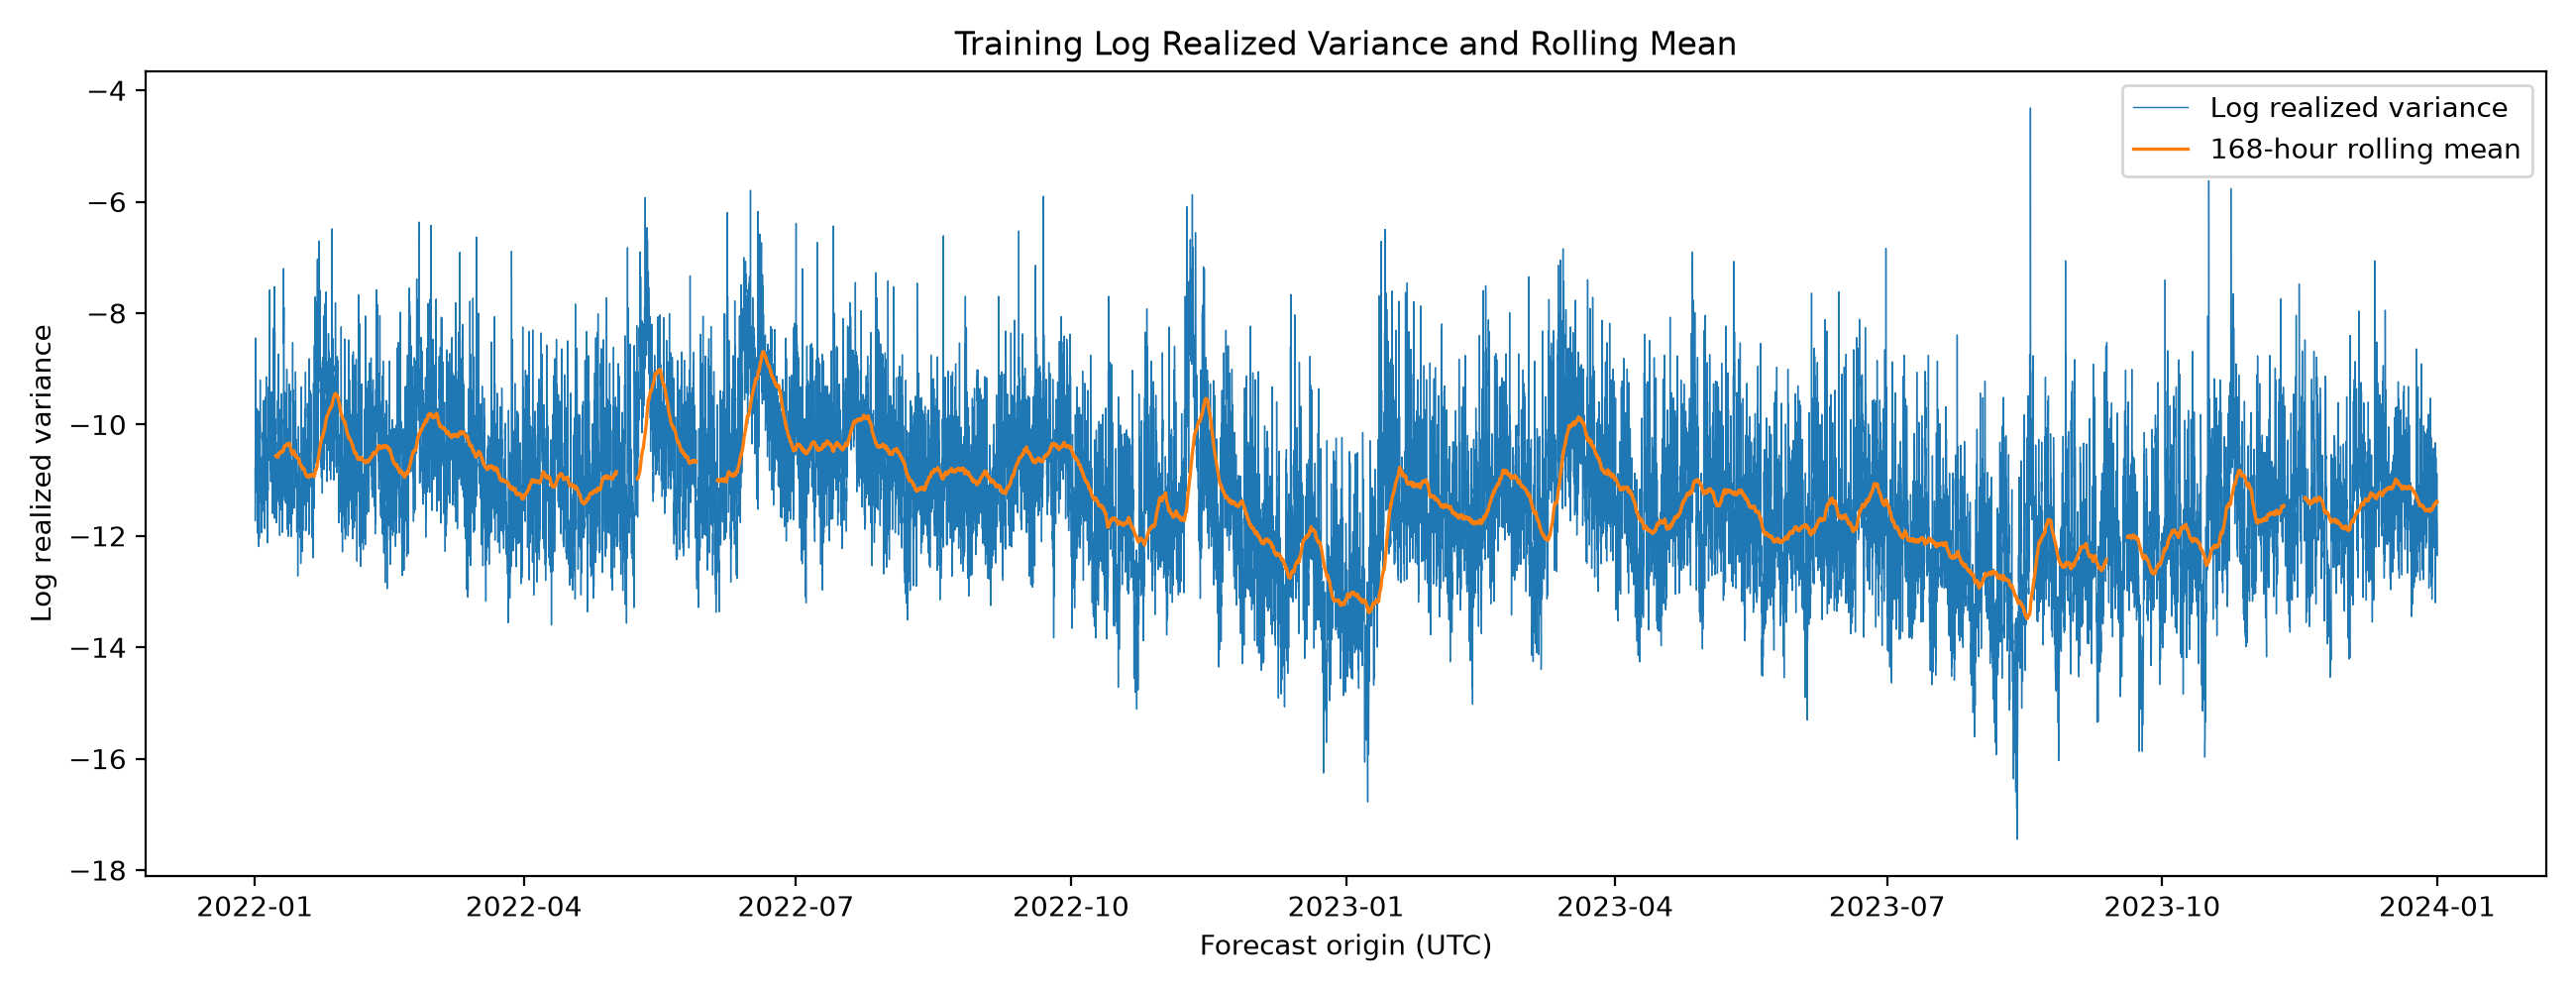
\includegraphics[
    width=0.95\textwidth
]
{../outputs/figures/training_log_rv_and_rolling_mean.png}
\caption{
Training-period log realized variance and its 168-hour
rolling mean
}
\label{fig:training-log-rv}
\end{figure}
}
{}

Log realized variance repeatedly returns toward its prevailing
level after large increases, indicating mean-reverting
behavior. The rolling mean nevertheless changes over the
training period, suggesting that the unconditional level is
not constant throughout the sample.

Table~\ref{tab:stationarity-tests} reports the formal test
results.

\begin{table}[H]
\centering
\caption{Training-period stationarity tests}
\label{tab:stationarity-tests}
\begin{tabular}{lrrrrl}
\toprule
Test
& Statistic
& \(p\)-value
& Lags
& Observations
& Decision at 5\% \\
\midrule
ADF
& -8.0186
& \(<0.001\)
& 40
& 11,277
& Reject unit root \\

KPSS
& 5.9013
& 0.010
& 57
& 11,318
& Reject level stationarity \\
\bottomrule
\end{tabular}
\end{table}

The augmented Dickey--Fuller test strongly rejects the
unit-root null \citep{saiddickey1984}, providing evidence of
mean reversion. The KPSS test also rejects global level
stationarity \citep{kpss1992}. Taken together, the results
indicate a persistent and mean-reverting series whose level or
dependence structure changes over longer periods.

These findings support the use of a fixed autoregression as a
forecasting benchmark while also motivating a specification
that allows gradual parameter variation.

\IfFileExists
{../outputs/figures/training_log_rv_acf.png}
{
\begin{figure}[H]
\centering
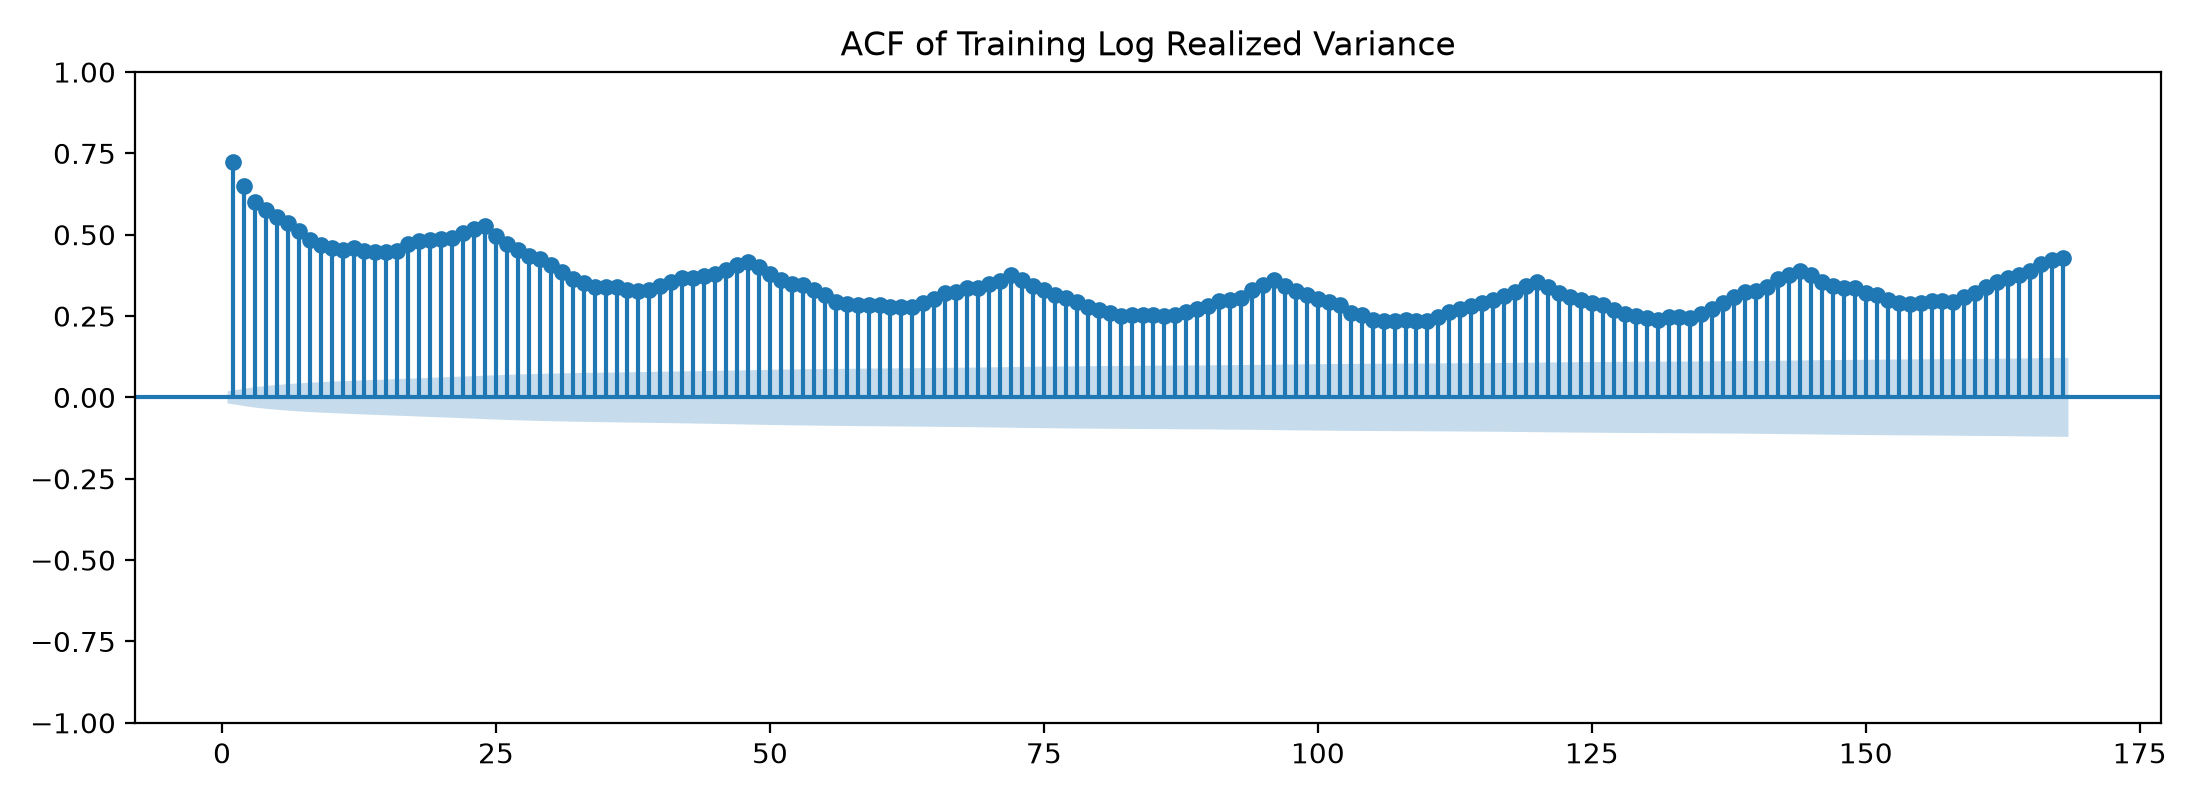
\includegraphics[
    width=0.92\textwidth
]
{../outputs/figures/training_log_rv_acf.png}
\caption{
Autocorrelation function of training-period log realized
variance
}
\label{fig:training-acf}
\end{figure}
}
{}

Figure~\ref{fig:training-acf} shows substantial
autocorrelation beyond the first few hours. The persistence
benchmark therefore captures only part of the temporal
dependence in hourly volatility.

\subsection{Autoregressive Order Selection}

AR orders from 1 through 24 are estimated on the training
sample and ranked by validation QLIKE. Table
\ref{tab:ar-order-selection} reports the five leading
specifications.

\begin{table}[H]
\centering
\caption{Leading AR specifications ranked by validation QLIKE}
\label{tab:ar-order-selection}
\begin{tabular}{rrrrrr}
\toprule
Order
& Training AIC
& Training BIC
& Validation MAE
& Validation RMSE
& Validation QLIKE \\
\midrule
24 & 43,353.53 & 43,546.57 & 0.6219 & 0.8023 & 0.5105 \\
23 & 43,392.98 & 43,578.29 & 0.6232 & 0.8037 & 0.5122 \\
22 & 43,455.91 & 43,633.50 & 0.6253 & 0.8061 & 0.5143 \\
21 & 43,528.03 & 43,697.90 & 0.6267 & 0.8080 & 0.5161 \\
20 & 43,557.89 & 43,720.04 & 0.6277 & 0.8090 & 0.5196 \\
\bottomrule
\end{tabular}
\end{table}

AR(24) achieves the lowest validation QLIKE, RMSE, and MAE
and is selected as the autoregressive benchmark. Its position
at the upper boundary of the candidate set suggests that
information from the preceding 24 hours remains useful. The
incremental gains decline as the order increases, indicating
that predictive dependence is distributed across several lags
rather than concentrated in a single hour.

The validation losses for AR(24) are \(0.6219\) for MAE,
\(0.8023\) for RMSE, and \(0.5105\) for QLIKE. Relative to
persistence, these values represent reductions of
approximately \(13.14\%\), \(12.59\%\), and \(21.22\%\),
respectively. Estimated lag dynamics therefore provide
substantial predictive value beyond the current volatility
level.

\subsubsection{AR Stability and Residual Diagnostics}

All characteristic roots of AR(24) lie outside the unit
circle. The minimum root modulus is \(1.0084\), indicating a
stable but highly persistent specification.

The first-order residual autocorrelation is \(0.0036\).
Ljung--Box portmanteau tests nevertheless reject residual white
noise at lags 29, 48, and 168, with \(p\)-values below
\(0.001\) \citep{ljungbox1978}.

AR(24) captures most immediate dependence but leaves weaker
correlation at longer horizons. It therefore provides a strong
forecasting benchmark while leaving scope for the
multi-horizon HAR-X specification.

\subsection{Fixed HAR-X Estimation Results}

Fixed HAR-X combines multi-horizon volatility components with
downside semivariance, trading activity, and aggressive-buying
information. Table~\ref{tab:fixed-harx-coefficients} reports
standardized coefficients with Newey--West HAC standard errors
\citep{neweywest1987}.

\begin{table}[H]
\centering
\caption{
Fixed HAR-X standardized coefficients with HAC(24) inference
}
\label{tab:fixed-harx-coefficients}
\scriptsize
\begin{tabular}{p{5.7cm}rrrr}
\toprule
Predictor
& Coefficient
& HAC standard error
& \(t\)-statistic
& \(p\)-value \\
\midrule
Current-hour volatility
& 0.2616
& 0.0239
& 10.94
& \(<0.001\) \\

Six-hour volatility
& 0.2632
& 0.0167
& 15.73
& \(<0.001\) \\

Twenty-four-hour volatility
& 0.2574
& 0.0183
& 14.09
& \(<0.001\) \\

One-hundred-sixty-eight-hour volatility
& 0.1163
& 0.0140
& 8.31
& \(<0.001\) \\

Transformed downside semivariance
& -0.0062
& 0.0192
& -0.32
& 0.745 \\

Log number of trades
& 0.3379
& 0.0153
& 22.13
& \(<0.001\) \\

Aggressive-buying proxy
& -0.0006
& 0.0088
& -0.07
& 0.948 \\
\bottomrule
\end{tabular}
\end{table}

All four HAR components have positive and statistically
significant coefficients, consistent with the
heterogeneous-horizon representation of realized volatility
\citep{corsi2009}. Current, intraday, daily, and weekly
volatility each contribute information after conditioning on
the remaining predictors.

Trading activity has a coefficient of \(0.3379\) and is highly
significant. Because the predictors are standardized, a
one-standard-deviation increase in log trade count is
associated with an increase of approximately \(0.338\) in
next-hour log realized variance, conditional on the other
variables.

This result is consistent with the information-arrival
interpretation of trading activity \citep{clark1973} and the
documented relationship between transaction counts and
volatility \citep{jones1994}. Among the three additional
market-activity variables, trade count provides the strongest
incremental predictive evidence.

The coefficients on downside semivariance and aggressive
buying are small and statistically insignificant. Their
average conditional associations with next-hour volatility are
therefore weak over the estimation period.

All coefficient estimates are interpreted as predictive
associations.

\subsection{Fixed HAR-X Validation Performance}

Table~\ref{tab:validation-model-comparison} compares the four
models on the validation sample.

\begin{table}[H]
\centering
\caption{Validation-period forecast performance}
\label{tab:validation-model-comparison}
\begin{tabular}{lrrrr}
\toprule
Model
& MAE
& RMSE
& QLIKE
& QLIKE improvement vs.\ Naive \\
\midrule
Naive
& 0.7160
& 0.9179
& 0.6480
& 0.00\% \\

AR(24)
& 0.6219
& 0.8023
& 0.5105
& 21.22\% \\

Fixed HAR-X
& 0.6106
& 0.7913
& 0.5083
& 21.56\% \\

TVP-HAR-X
& 0.6079
& 0.7857
& 0.4864
& 24.93\% \\
\bottomrule
\end{tabular}
\end{table}

Fixed HAR-X improves on AR(24) under all three metrics. The
QLIKE reduction is \(0.42\%\), showing that AR(24) already
captures much of the predictive content in recent volatility.

Fixed HAR-X achieves this performance with seven structured
predictors and incorporates information extending to the
preceding week. The specification therefore provides a
parsimonious and interpretable alternative to a larger set of
individual hourly lags.

Its residual first-order autocorrelation is close to zero, and
the Durbin--Watson statistic is \(2.009\). Ljung--Box tests
remain significant at lags 24, 48, and 168, indicating
residual dependence at longer horizons.

\subsection{TVP-HAR-X Parameter Estimates}

The TVP-HAR-X variance parameters are estimated on the
training sample by maximizing the Kalman-filter
prediction-error likelihood \citep{durbin2012}. Three sets of
starting values converge to nearly identical solutions,
indicating numerical stability.

\begin{table}[H]
\centering
\caption{Training-period TVP-HAR-X variance parameters}
\label{tab:tvp-variance-parameters}
\begin{tabular}{lrr}
\toprule
Parameter
& Variance
& Standard deviation \\
\midrule
Observation disturbance
& \(7.4918\times10^{-1}\)
& \(8.6555\times10^{-1}\) \\

Intercept-state innovation
& \(2.5406\times10^{-5}\)
& \(5.0404\times10^{-3}\) \\

Common slope-state innovation
& \(1.6681\times10^{-6}\)
& \(1.2915\times10^{-3}\) \\
\bottomrule
\end{tabular}
\end{table}

Both state innovation variances are small relative to the
observation variance, producing gradual coefficient movement.
The intercept innovation standard deviation exceeds the common
slope innovation standard deviation, indicating faster
variation in the overall volatility level than in the marginal
predictor effects.

The estimated state variances are positive, so the fitted model
does not collapse numerically to a fixed-coefficient
specification.

\subsection{Time-Varying Coefficient Behavior}

Table~\ref{tab:tvp-state-summary} summarizes the predicted
state estimates during validation.

\begin{table}[H]
\centering
\caption{Validation-period time-varying coefficient summary}
\label{tab:tvp-state-summary}
\scriptsize
\begin{tabular}{p{5.3cm}rrrr}
\toprule
State
& Mean
& Standard deviation
& Minimum
& Maximum \\
\midrule
Intercept
& -11.2035
& 0.0936
& -11.4340
& -10.9837 \\

Current-hour volatility
& 0.1102
& 0.0312
& 0.0502
& 0.1918 \\

Six-hour volatility
& 0.2447
& 0.0194
& 0.1988
& 0.2976 \\

Twenty-four-hour volatility
& 0.1721
& 0.0271
& 0.1203
& 0.2514 \\

One-hundred-sixty-eight-hour volatility
& 0.0076
& 0.0316
& -0.0781
& 0.0576 \\

Transformed downside semivariance
& -0.0175
& 0.0508
& -0.1261
& 0.0787 \\

Log number of trades
& 0.5336
& 0.0528
& 0.4407
& 0.6513 \\

Aggressive-buying proxy
& -0.0324
& 0.0232
& -0.0864
& 0.0373 \\
\bottomrule
\end{tabular}
\end{table}

Trading activity has the largest average positive coefficient
and remains positive throughout validation, ranging from
approximately \(0.441\) to \(0.651\). It is therefore a
consistently informative predictor within this period.

The six-hour and twenty-four-hour coefficients also remain
positive and vary within relatively narrow ranges. Short- and
medium-horizon volatility persistence is consequently stable
during validation.

The weekly coefficient fluctuates around zero, while the
downside-semivariance and aggressive-buying coefficients
change sign. Their predictive contributions vary more
substantially across the sample.

The state paths describe changes in conditional forecasting
relationships and are not assigned a causal interpretation.

\subsection{TVP-HAR-X Validation Performance}

TVP-HAR-X records validation MAE of \(0.6079\), RMSE of
\(0.7857\), and QLIKE of \(0.4864\). QLIKE is \(4.30\%\)
lower than for Fixed HAR-X and \(24.93\%\) lower than for the
persistence benchmark.

The standardized innovations have a mean of approximately
\(-0.0095\), a standard deviation of \(1.024\), and
first-order autocorrelation of \(0.0007\). These values are
close to the corresponding theoretical benchmarks of zero,
one, and zero.

Longer-horizon Ljung--Box tests remain significant. Given the
large diagnostic sample, these rejections reflect small
autocorrelations accumulated across several lags. The
state-space model improves validation forecasts while leaving
some temporal dependence unexplained.

\subsection{Final Out-of-Sample Test Results}

After model selection, AR(24), Fixed HAR-X, and TVP-HAR-X
are re-estimated using the combined training and validation
sample. The locked specifications are then evaluated on
\(8{,}422\) common test observations from 2025.

Table~\ref{tab:final-test-results} reports the final
out-of-sample performance.

\begin{table}[H]
\centering
\caption{Final 2025 test-set forecast performance}
\label{tab:final-test-results}
\begin{tabular}{lrrrrrr}
\toprule
Model
& MAE
& MAE rank
& RMSE
& RMSE rank
& QLIKE
& QLIKE rank \\
\midrule
Naive
& 0.7021
& 4
& 0.9101
& 4
& 0.7007
& 4 \\

AR(24)
& 0.6133
& 3
& 0.7997
& 3
& 0.5054
& 3 \\

Fixed HAR-X
& 0.5980
& 2
& 0.7807
& 2
& \textbf{0.4764}
& \textbf{1} \\

TVP-HAR-X
& \textbf{0.5901}
& \textbf{1}
& \textbf{0.7734}
& \textbf{1}
& 0.4800
& 2 \\
\bottomrule
\end{tabular}
\end{table}

All three estimated models improve substantially on
persistence. Relative to Naive, test QLIKE falls by
\(27.87\%\) for AR(24), \(32.02\%\) for Fixed HAR-X, and
\(31.50\%\) for TVP-HAR-X.

Fixed HAR-X reduces QLIKE by \(5.75\%\) relative to AR(24).
The structured multi-horizon and market-activity predictors
therefore provide additional forecasting information beyond
the 24 hourly lags.

The ranking of the two HAR-X models varies across loss
functions. TVP-HAR-X records the lowest MAE and RMSE, while
Fixed HAR-X records the lowest QLIKE. Relative to Fixed HAR-X,
TVP-HAR-X reduces absolute error by \(1.33\%\) and squared
error by \(1.87\%\). Its QLIKE is \(0.76\%\) higher.

\IfFileExists
{../outputs/figures/final_test_mae_comparison.png}
{
\begin{figure}[H]
\centering
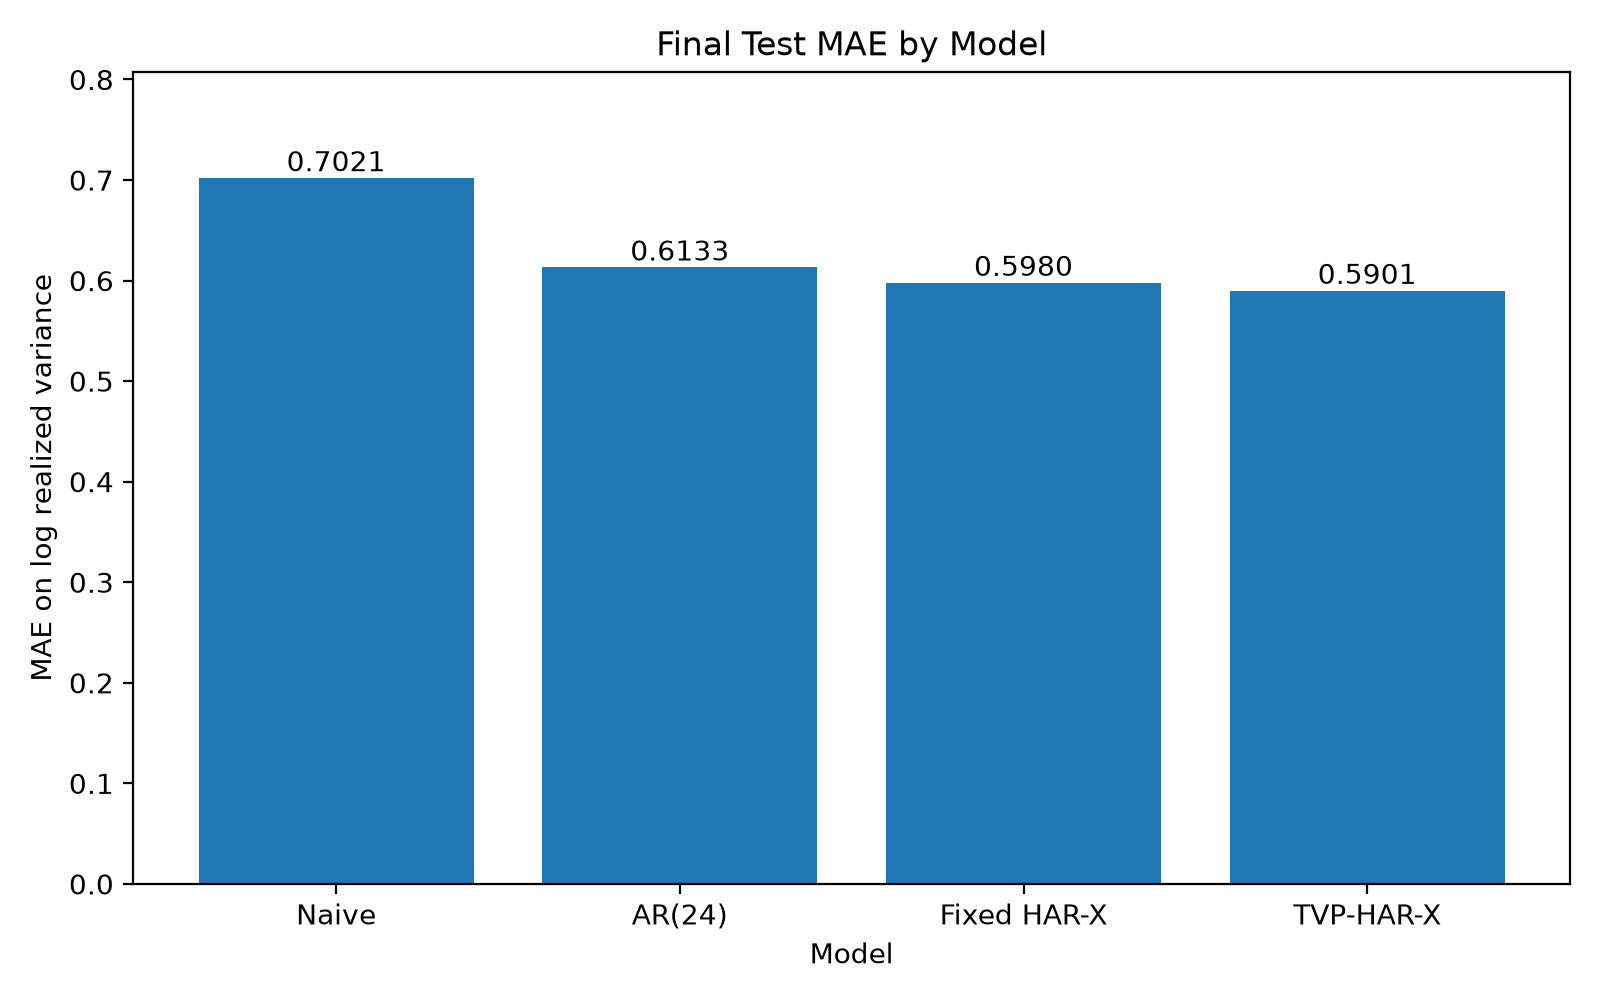
\includegraphics[
    width=0.80\textwidth
]
{../outputs/figures/final_test_mae_comparison.png}
\caption{Final test MAE across forecasting models}
\label{fig:final-mae}
\end{figure}
}
{}

\IfFileExists
{../outputs/figures/final_test_rmse_comparison.png}
{
\begin{figure}[H]
\centering
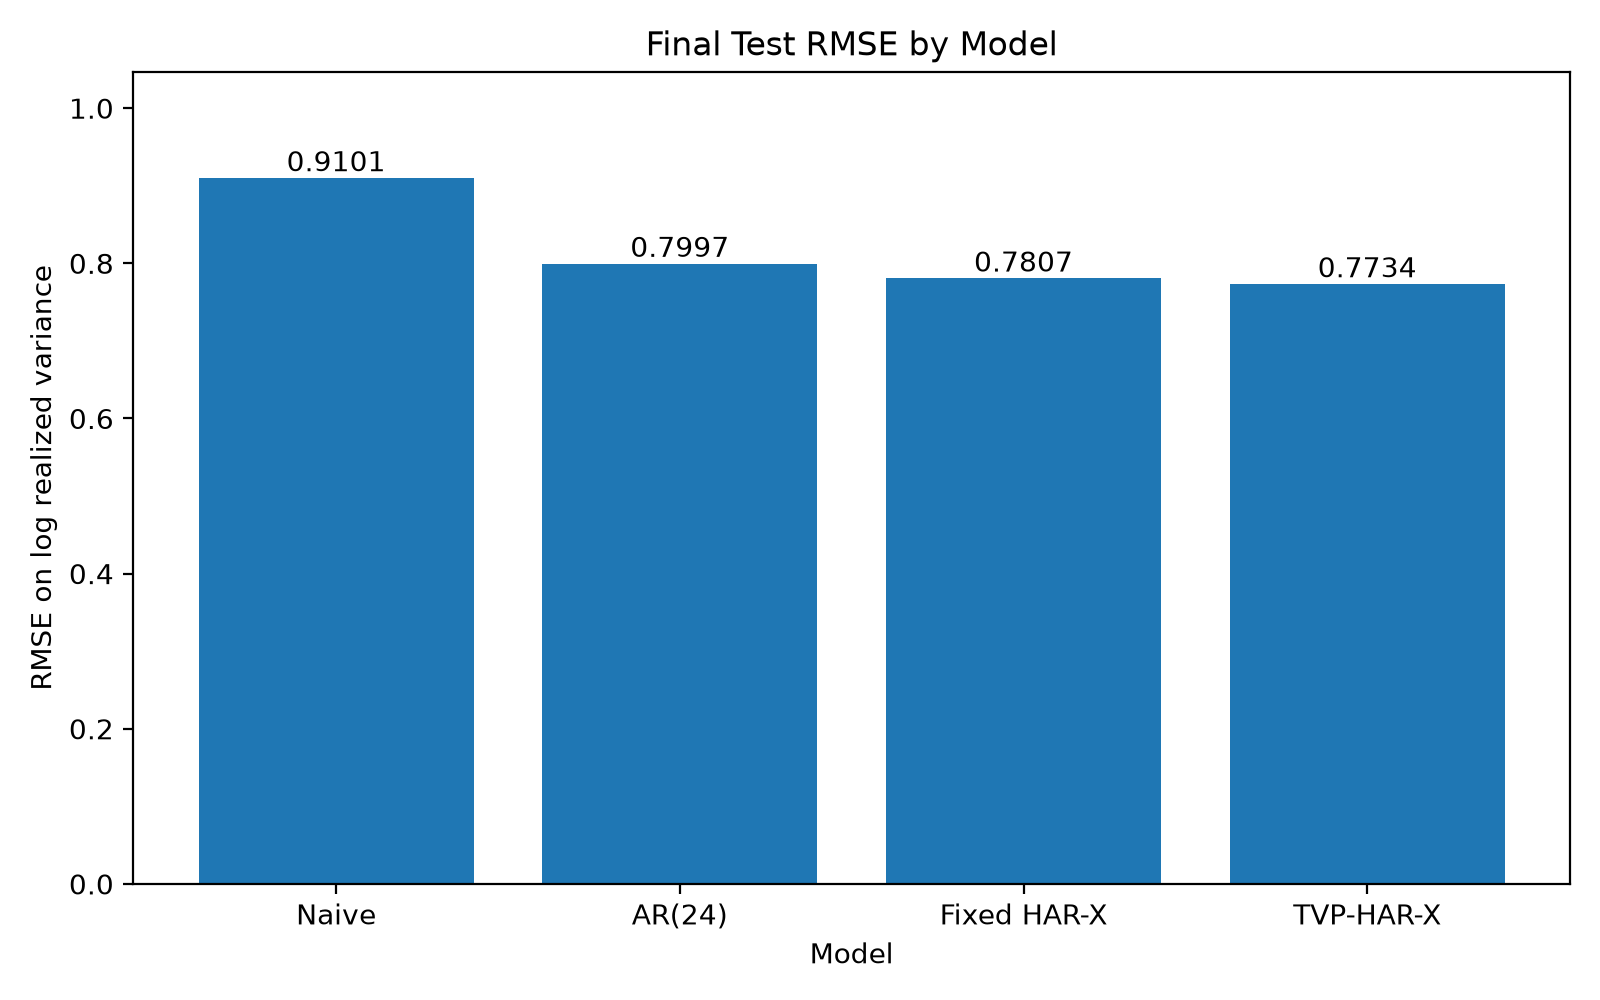
\includegraphics[
    width=0.80\textwidth
]
{../outputs/figures/final_test_rmse_comparison.png}
\caption{Final test RMSE across forecasting models}
\label{fig:final-rmse}
\end{figure}
}
{}

\IfFileExists
{../outputs/figures/final_test_qlike_comparison.png}
{
\begin{figure}[H]
\centering
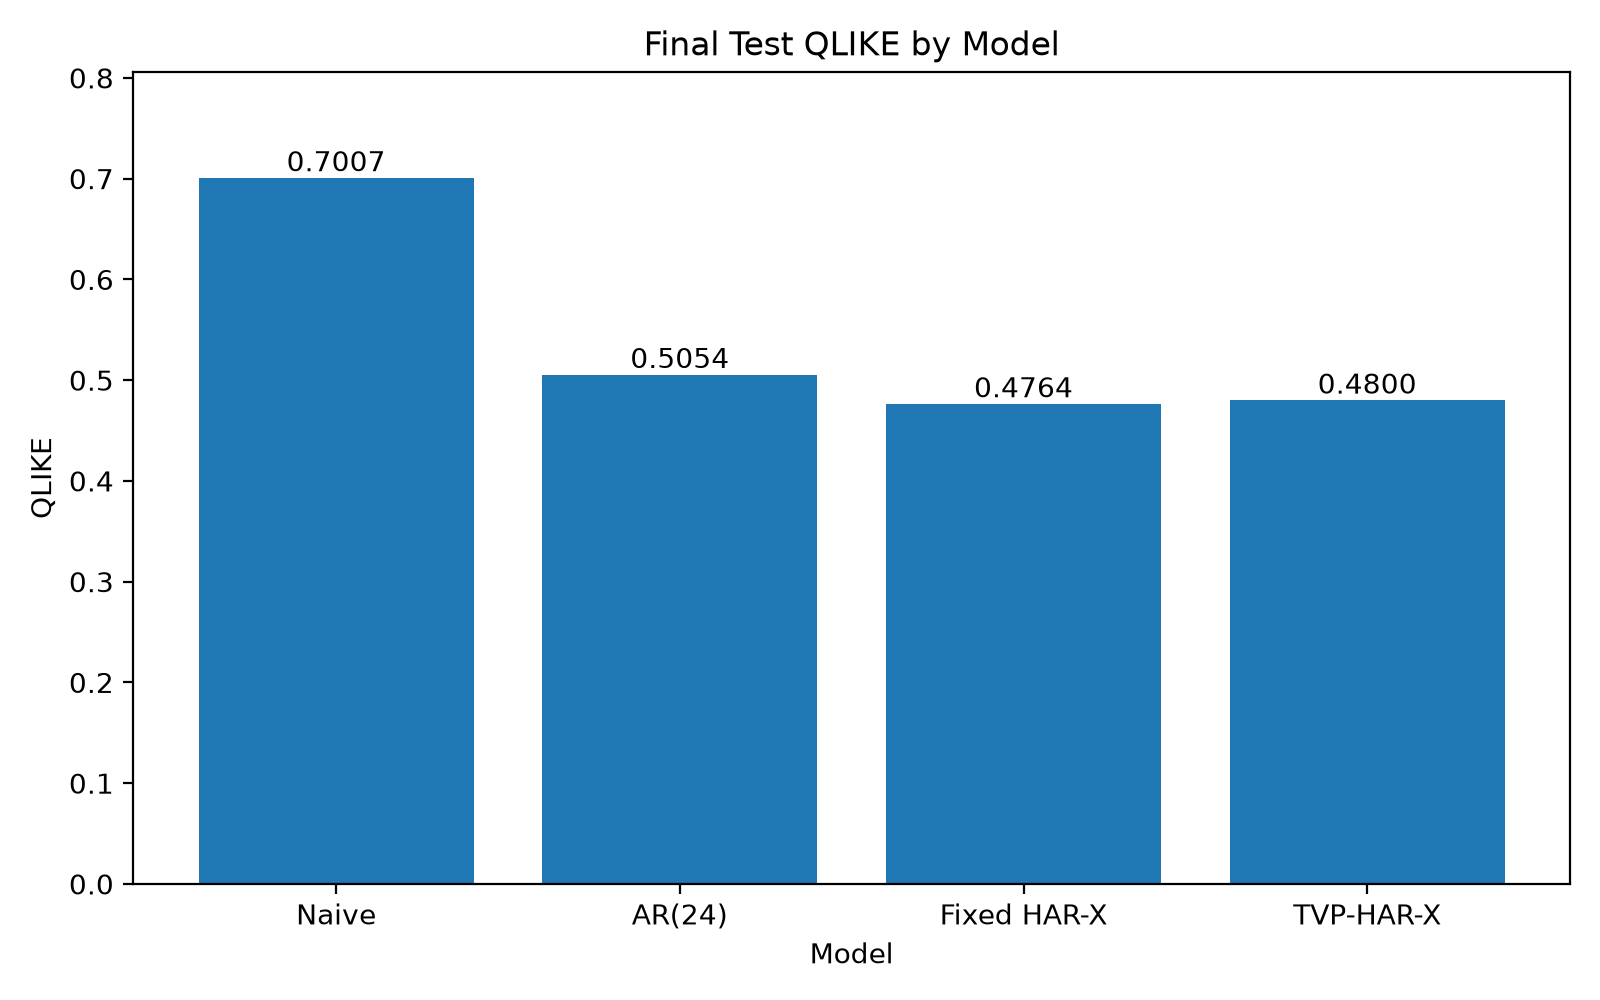
\includegraphics[
    width=0.80\textwidth
]
{../outputs/figures/final_test_qlike_comparison.png}
\caption{Final test QLIKE across forecasting models}
\label{fig:final-qlike}
\end{figure}
}
{}

Figures~\ref{fig:final-mae}--\ref{fig:final-qlike} show that
the difference between the two HAR-X specifications is small
relative to their gains over Naive and AR(24). They also
illustrate the change in ranking between log-scale errors and
variance-scale loss.

\subsection{Predictive-Loss Significance Tests}

Table~\ref{tab:tvp-fixed-loss-tests} reports
Diebold--Mariano-type loss-differential tests
\citep{dieboldmariano1995} using Newey--West HAC standard
errors \citep{neweywest1987}. The loss differential is defined
so that positive values favor TVP-HAR-X.

\begin{table}[H]
\centering
\caption{
HAC loss-differential tests:
TVP-HAR-X versus Fixed HAR-X
}
\label{tab:tvp-fixed-loss-tests}
\begin{tabular}{lrrrrl}
\toprule
Loss
& Fixed HAR-X
& TVP-HAR-X
& Improvement
& Test statistic
& One-sided \(p\)-value \\
\midrule
Absolute error
& 0.5980
& 0.5901
& 1.33\%
& 6.2596
& \(<0.001\) \\

Squared error
& 0.6096
& 0.5981
& 1.87\%
& 6.0210
& \(<0.001\) \\

QLIKE
& 0.4764
& 0.4800
& -0.76\%
& -1.2118
& 0.887 \\
\bottomrule
\end{tabular}
\end{table}

TVP-HAR-X significantly reduces absolute and squared loss
relative to Fixed HAR-X. The corresponding one-sided
\(p\)-values are below \(0.001\).

The QLIKE loss differential has a mean of \(-0.00362\) and a
one-sided \(p\)-value of \(0.887\). The test therefore provides
no evidence that TVP-HAR-X improves on Fixed HAR-X under the
pre-specified primary loss. The negative point estimate is
consistent with the lower QLIKE reported for Fixed HAR-X.

TVP-HAR-X also improves significantly on Naive and AR(24)
under all three losses. Its test QLIKE is approximately
\(5.03\%\) lower than that of AR(24), with a one-sided
\(p\)-value below \(0.001\).

\subsection{Validation--Test Comparison}

The relative performance of Fixed HAR-X and TVP-HAR-X changes
between the validation and test periods. TVP-HAR-X reduces
validation QLIKE by \(4.30\%\) relative to Fixed HAR-X, whereas
its test QLIKE is \(0.76\%\) higher.

This change in ranking shows that the validation advantage of
the time-varying specification does not persist uniformly
through the test period.

\IfFileExists
{../outputs/figures/final_test_monthly_qlike.png}
{
\begin{figure}[H]
\centering
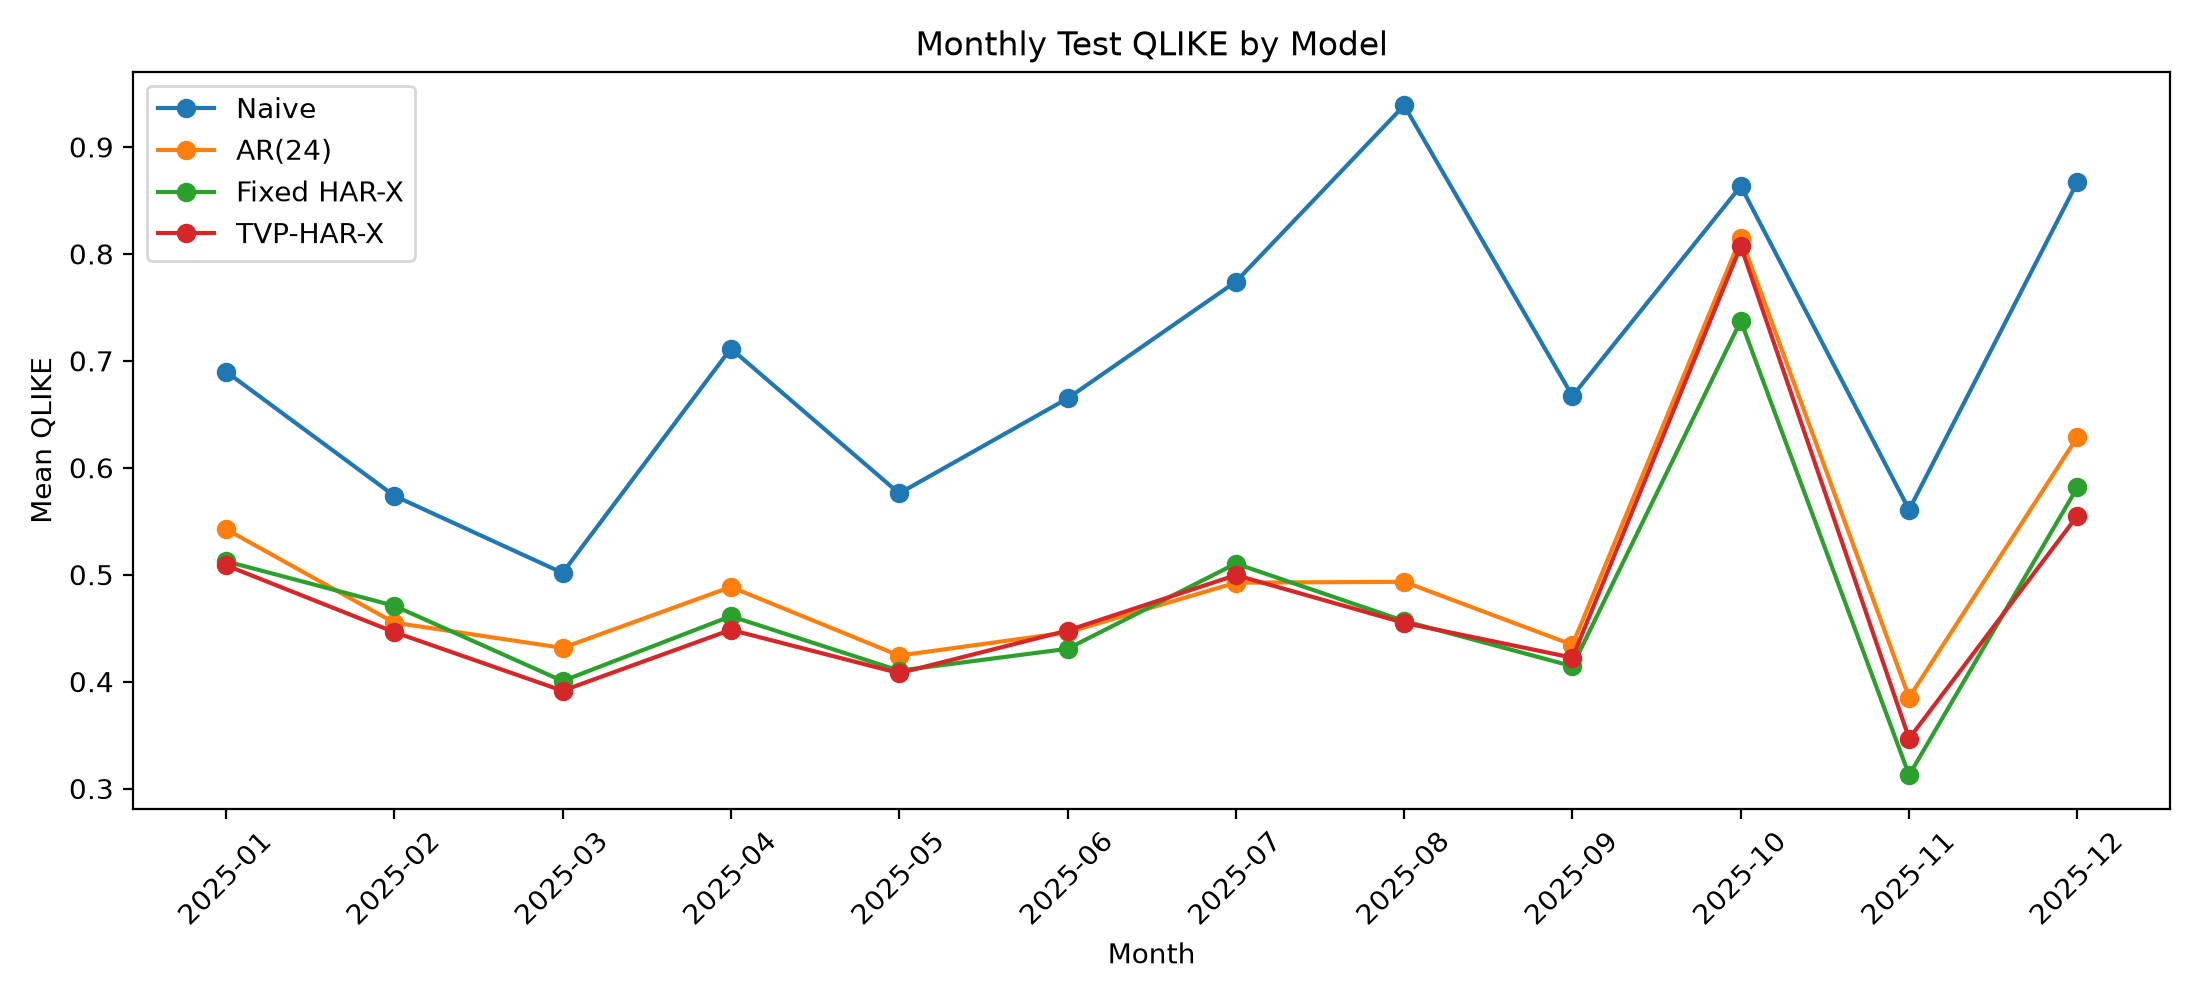
\includegraphics[
    width=0.94\textwidth
]
{../outputs/figures/final_test_monthly_qlike.png}
\caption{Monthly test-period QLIKE by model}
\label{fig:monthly-qlike}
\end{figure}
}
{}

Figure~\ref{fig:monthly-qlike} reports monthly QLIKE during
2025. The ranking of Fixed HAR-X and TVP-HAR-X varies across
months, so the annual averages combine periods with different
relative performance.

\IfFileExists
{../outputs/figures/final_test_cumulative_qlike_difference_fixed_vs_tvp.png}
{
\begin{figure}[H]
\centering
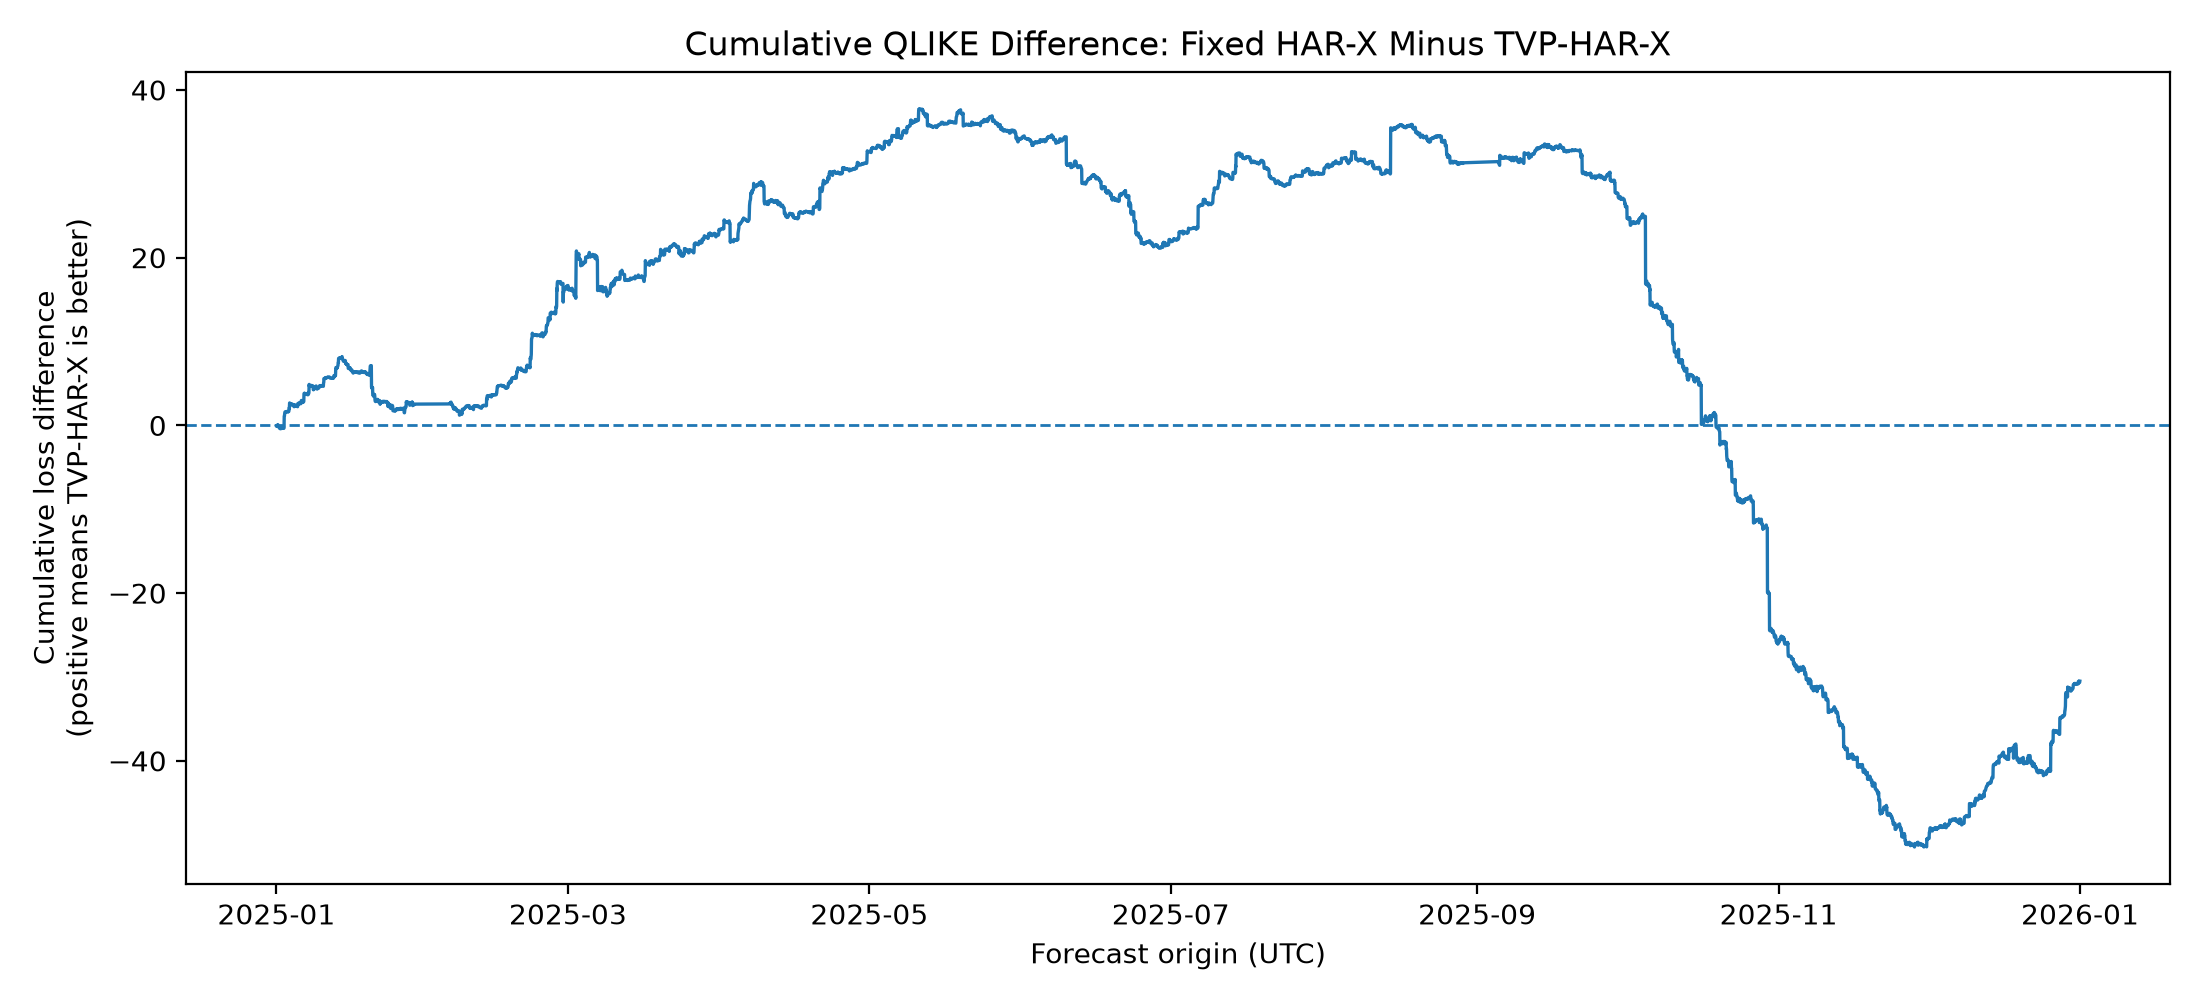
\includegraphics[
    width=0.94\textwidth
]
{../outputs/figures/final_test_cumulative_qlike_difference_fixed_vs_tvp.png}
\caption{
Cumulative QLIKE difference between Fixed HAR-X and TVP-HAR-X
}
\label{fig:cumulative-qlike-difference}
\end{figure}
}
{}

Figure~\ref{fig:cumulative-qlike-difference} displays the
cumulative difference between Fixed HAR-X and TVP-HAR-X
QLIKE. An upward segment indicates lower loss for TVP-HAR-X,
while a downward segment indicates lower loss for Fixed HAR-X.
The path confirms that neither specification maintains a
uniform advantage throughout the test year.

\subsection{Summary of Empirical Findings}

The empirical results yield five main findings.

\begin{enumerate}[label=(\arabic*)]

    \item
    Hourly log realized variance is persistent and mean
    reverting, although global level stationarity is rejected.

    \item
    AR(24) improves substantially on persistence, indicating
    that predictive dependence extends across several recent
    hours.

    \item
    Fixed HAR-X improves on AR(24), particularly under test
    QLIKE, supporting the use of multi-horizon volatility and
    market-activity predictors.

    \item
    Trading activity provides the strongest incremental
    predictor among the additional HAR-X variables.

    \item
    TVP-HAR-X achieves the lowest MAE and RMSE, while Fixed
    HAR-X achieves the lowest QLIKE. The gains from parameter
    variation therefore depend on the evaluation criterion.

\end{enumerate}

The strongest and most stable improvement arises from moving
from persistence and AR(24) to the HAR-X information set.
Time-varying coefficients provide additional gains in
log-scale forecast accuracy, while the fixed specification
performs best under the primary variance-scale loss.